
\begin{figure}[ht]
  \centering
  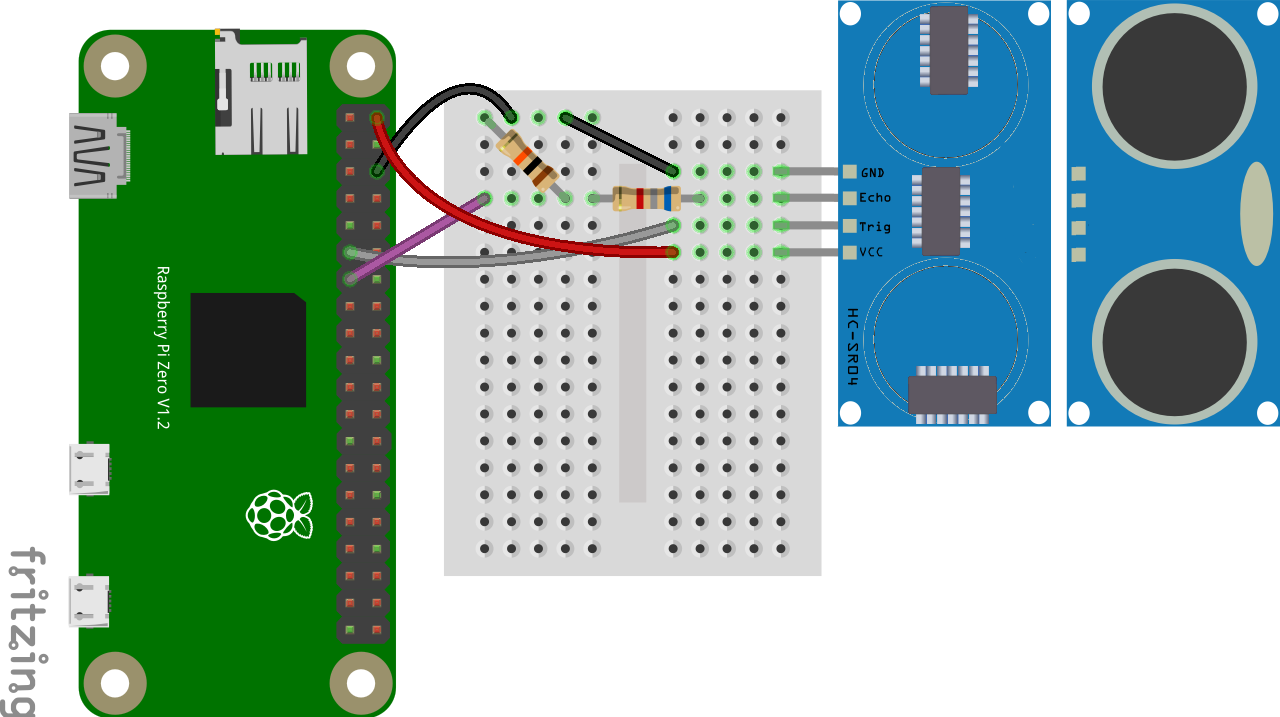
\includegraphics[scale=0.25]{images/HC-SR04_Steckplatine.png}	
  %	\caption{}
  \label{DHT22_Steckplatine}
\end{figure}

\begin{figure}[ht]
	\centering
	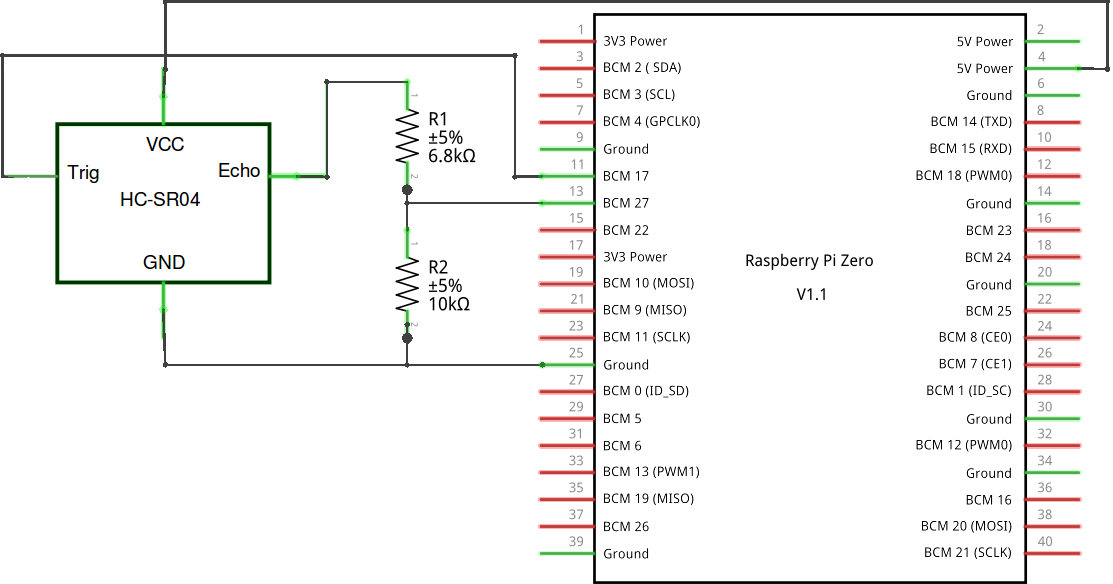
\includegraphics[scale=0.25]{images/HC-SR04_Schaltplan.png}	
	%	\caption{}
	\label{DHT22_Steckplatine}
\end{figure}

\ExerciseBox{
Miss die Distanz [Beispiele]\\
Filtere die gemessene Distanz\\
Ermittle die Geschwindigkeit eines bewegten Objektes\\
Bewerte die Distanz mit der Ampel: Rot niedriger Abstand, Gr�n ausreichender Abstand     
Gib den Wert zyklisch am TM1637 Display aus [Beispiel Python]\\
Verwende die korrigierte Schallgeschwindingkeit bei aktueller Lufttemperatur vom DHT22}


\subsubsection{C}

\begin{console}
	cd ~/Projekte
	git clone https://github.com/mstroh76/Sensors-WiringPi.git
	cd Sensors-WiringPi/HC-SR04	
	g++ -o HC-SR04 *.cpp -lwiringPi	
	./HC-SR04
	cd ..
	geany HC-SR04.geany &
\end{console}


\subsubsection{C\#}

\begin{console}
	cd ~/Projekte
	git clone https://github.com/chirndler/wiringpi.net.sensors.git
	cd wiringpi.net.sensors
	xbuild /p:Configuration=Release wiringpi.net.sensors.sln
	cd bin/Release/
	sudo mono wiringpi.net.sensors.sample.exe 2
\end{console}


\subsubsection{Python}

\lstset{language=Python, caption=, 
        label=HCSR04Program, frame=single, basicstyle=\ttfamily
	      \footnotesize, breakatwhitespace=false, showstringspaces=false, 
        showtabs=false, tabsize=2 }
\lstinputlisting{source/HC_SR04.py}

\begin{console}
	python3 HC_SR04.py
\end{console}


\subsubsection{Blockly-gPIo}

\begin{figure}[ht]
	\centering
	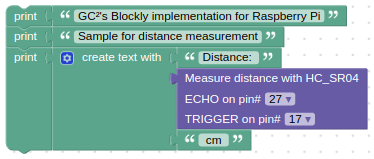
\includegraphics[scale=0.6]{images/Blockly-gPIo_HC_SR04.png}
	%	\caption{}
	\label{Blockly-gPIo_HC_SR04}
\end{figure}

